\subsection{Results}


During the course of the diary study, we collected $868$ search entries with an average of 27 entries per person. 9\% of searches (33 out of 868) failed, not providing users with the information they sought. About a third (279 out of 868 search entries) were difficult (opposed to `easy' described below). 41.2\% used Google app, 49.4\% used a specific url, and the rest used other apps (i.e Amazon app). Participants performed an average of $1.2$ searches ($median=1, min =1, max=5$) and followed $2.5$ links ($median=2, min=0, max=39$) to find their information. Participants evaluated the task difficulty at an average of $1.9$ ($median=2,  \sigma=1, min=1, max=5$) based on a Likert scale with 1 being very easy and 5 being very difficult. 

The search queries were analyzed from 2 different perspectives. First, whether the queries were imprecise or precise. We define imprecise queries to consist of 2 or more intermediate queries or 3 or more links clicked. Otherwise, the queries were classified to be precise. Second, whether the queries were difficult or easy. Too hard indicates failed, with a difficulty rating of $4$ or $5$, or more than $2$ minutes of work. Otherwise, the queries were classified to be easy. 

Using these two classifiers, were were able to bin the queries into $4$ categories: We found that 49 \% of the queries were precise and easy, 7 \% were precise and difficult, 20 \% were imprecise and easy, and 24 \% were imprecise and difficult. Table 1 shows various examples for these $4$ categories.

From the results, we distill a number of key findings: Although search was usually successful, it was difficult about a third of the time (31\%), especially when search was more imprecise. Mobile search using imprecise queries is a real problem, and most difficulty users have is with these queries. Further, most of these imprecise and difficult searches involve refinements to querying relationships between entities in search such as movies to cast on \url{www.imdb.com} or recipe ingredients to dishes on \url{allrecipes.com}.

In sum, we believe the large majority of searches could have benefited from a tool that helped users navigate through the information neighborhoods typical of imprecise search. 

% Vidya: I don't think these two paras are relevant to this paper.

%The average time taken to record a search activity was $131.6$ seconds ($median=120, max=1200$). 
%People use applications more than websites for certain activities. On an average, 18.5\% (160 out of 868) of the searches were using applications than web portals. The most popular category searched using an application was \emph{shopping} (47\%). Surprisingly, participants frequently knew the exact keyword to put in as a search phrase. People use mobile apps for regular, standard search activities (i.e. weather, shopping, location, names, exchange rate, bus route, definition). For less frequent, more complicated searches, they will try it on a web portal but easily give up because of the screen size restriction and choose another method (i.e. go to their desktop, ask friends).

%
%We looked for duplicate themes from collected diary entries and did not start with a set of fixed categories. We adopted most of the categories from \cite{chi2008} and added new categories such as `\emph{how-to}', `\emph{unit conversion}', `\emph{definition}', and `\emph{name}'. There are 17 categories based on the diary entries.
%The \emph{how-to} category includes information about practical advice and detailed instruction of an activity. The \emph{unit conversion} includes kilometer to miles conversion, fahrenheit to celsius, and exchange rate. The \emph{definition} includes any need of terminology definition and detailed explanation. The \emph{name} includes search of a certain person or movie title. The largest category of collected entries was \emph{trivia} (51\%). They are the random thoughts from the participants such as ``story of shutter island". The second highest was \emph{shopping} (13\%), followed by \emph{point of interest} (10\%) and \emph{definition} (6\%).



%Vidya: I think this figure is hard to understand and looks too complicated.
%Figure \ref{fig:searchtype} categorizes search type of diary entries by success/failure, easy/difficult, open/specific queries, and hit or miss. Overall, the large blue section shows that people are mostly successful in finding information with their mobile device (though they may never attempt many challenging searches). About a third of searches are still difficult, and over half of difficult searches are open. 
%
%
%\begin{figure}[ht]
%\centering
%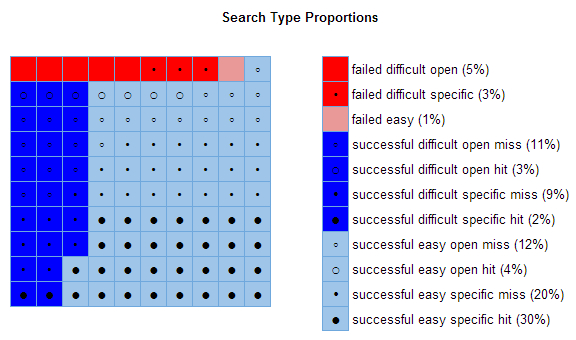
\includegraphics[width=3in]{images/searchtype}
%\caption{Search type by success/failure, easy/difficult, open/specific, and hit/miss. Blue: success, red: failure, saturated color: easy, bright color: difficult, empty dot: open, filled dot: specific, smaller dot: miss, bigger dot: hit}
%\label{fig:searchtype}
%\end{figure}




